\documentclass{standalone}
\usepackage{tikz}
\usetikzlibrary{patterns, positioning}
\usepackage[sfdefault]{ClearSans} %% option 'sfdefault' activates Clear Sans as the default text font
\usepackage[T1]{fontenc}

\begin{document}
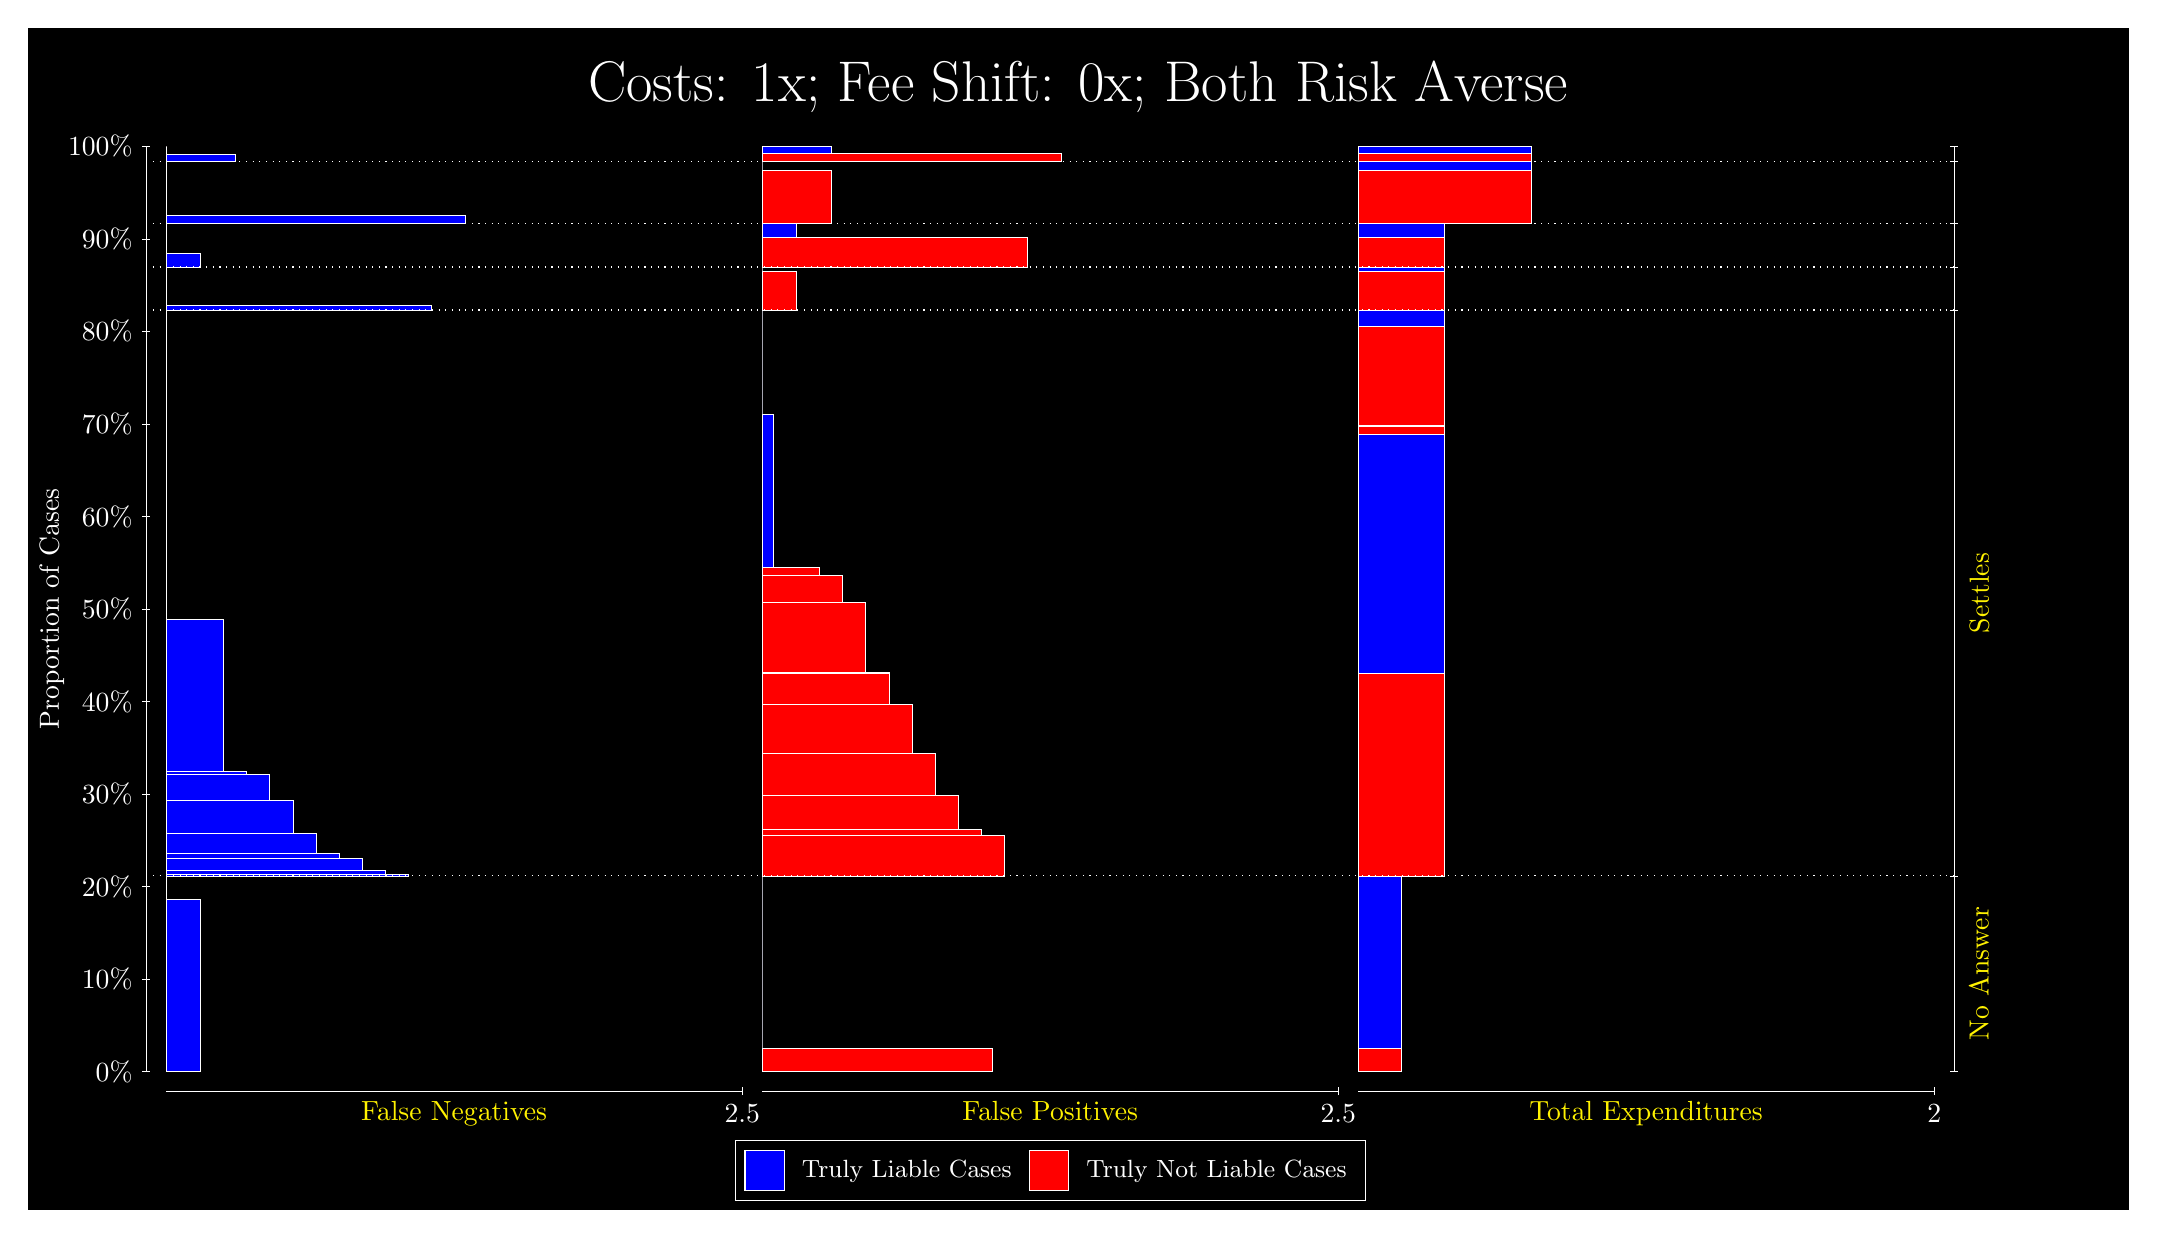
\begin{tikzpicture}
\draw[fill=black] (0,0) rectangle (26.667,15);
\draw[text=white] (0,13.5) rectangle (26.667,15) node[midway] {\huge Costs: 1x; Fee Shift: 0x; Both Risk Averse};
\draw[white, very thin] (1.5,1.75) -- (1.5,13.5);
\node[rotate=90, text=white, anchor=center] at (0.3, 7.625) {Proportion of Cases};
\draw[white, very thin] (1.45,1.75) -- (1.55,1.75);
\node[text=white, anchor=east] at (1.45, 1.75) {0\%};
\draw[white, very thin] (1.45,2.925) -- (1.55,2.925);
\node[text=white, anchor=east] at (1.45, 2.925) {10\%};
\draw[white, very thin] (1.45,4.1) -- (1.55,4.1);
\node[text=white, anchor=east] at (1.45, 4.1) {20\%};
\draw[white, very thin] (1.45,5.275) -- (1.55,5.275);
\node[text=white, anchor=east] at (1.45, 5.275) {30\%};
\draw[white, very thin] (1.45,6.45) -- (1.55,6.45);
\node[text=white, anchor=east] at (1.45, 6.45) {40\%};
\draw[white, very thin] (1.45,7.625) -- (1.55,7.625);
\node[text=white, anchor=east] at (1.45, 7.625) {50\%};
\draw[white, very thin] (1.45,8.8) -- (1.55,8.8);
\node[text=white, anchor=east] at (1.45, 8.8) {60\%};
\draw[white, very thin] (1.45,9.975) -- (1.55,9.975);
\node[text=white, anchor=east] at (1.45, 9.975) {70\%};
\draw[white, very thin] (1.45,11.15) -- (1.55,11.15);
\node[text=white, anchor=east] at (1.45, 11.15) {80\%};
\draw[white, very thin] (1.45,12.325) -- (1.55,12.325);
\node[text=white, anchor=east] at (1.45, 12.325) {90\%};
\draw[white, very thin] (1.45,13.5) -- (1.55,13.5);
\node[text=white, anchor=east] at (1.45, 13.5) {100\%};

\draw[white, very thin] (24.457,1.75) -- (24.457,13.5);
\draw[white, very thin] (24.407,1.75) -- (24.507,1.75);
\node[anchor=west] at (24.407, 1.75) {};
\draw[white, very thin] (24.407,4.2341) -- (24.507,4.2341);
\node[anchor=west] at (24.407, 4.2341) {};
\draw[white, very thin] (24.407,11.421) -- (24.507,11.421);
\node[anchor=west] at (24.407, 11.421) {};
\draw[white, very thin] (24.407,11.968) -- (24.507,11.968);
\node[anchor=west] at (24.407, 11.968) {};
\draw[white, very thin] (24.407,12.52) -- (24.507,12.52);
\node[anchor=west] at (24.407, 12.52) {};
\draw[white, very thin] (24.407,13.305) -- (24.507,13.305);
\node[anchor=west] at (24.407, 13.305) {};
\draw[white, very thin] (24.407,13.5) -- (24.507,13.5);
\node[anchor=west] at (24.407, 13.5) {};

\draw[white, very thin, fill=blue] (1.75,1.75) rectangle (2.1891,3.9353);
\draw[white, very thin, fill=red] (1.75,3.9353) rectangle (1.75,4.2341);
\draw[white, very thin, fill=blue] (1.75,4.2341) rectangle (4.8239,4.2493);
\draw[white, very thin, fill=blue] (1.75,4.2493) rectangle (4.5312,4.3066);
\draw[white, very thin, fill=blue] (1.75,4.3066) rectangle (4.2384,4.4545);
\draw[white, very thin, fill=blue] (1.75,4.4545) rectangle (3.9457,4.5209);
\draw[white, very thin, fill=blue] (1.75,4.5209) rectangle (3.6529,4.7706);
\draw[white, very thin, fill=blue] (1.75,4.7706) rectangle (3.3602,5.1951);
\draw[white, very thin, fill=blue] (1.75,5.1951) rectangle (3.0674,5.5225);
\draw[white, very thin, fill=blue] (1.75,5.5225) rectangle (2.7746,5.5593);
\draw[white, very thin, fill=blue] (1.75,5.5593) rectangle (2.4819,7.4958);
\draw[white, very thin, fill=red] (1.75,7.4958) rectangle (1.75,11.421);
\draw[white, very thin, fill=blue] (1.75,11.421) rectangle (5.1167,11.477);
\draw[white, very thin, fill=red] (1.75,11.477) rectangle (1.75,11.968);
\draw[white, very thin, fill=blue] (1.75,11.968) rectangle (2.1891,12.142);
\draw[white, very thin, fill=red] (1.75,12.142) rectangle (1.75,12.52);
\draw[white, very thin, fill=blue] (1.75,12.52) rectangle (5.5558,12.627);
\draw[white, very thin, fill=red] (1.75,12.627) rectangle (1.75,13.305);
\draw[white, very thin, fill=blue] (1.75,13.305) rectangle (2.6283,13.396);
\draw[white, very thin, fill=red] (1.75,13.396) rectangle (1.75,13.5);
\draw[white, very thin, fill=red] (9.3189,1.75) rectangle (12.246,2.0487);
\draw[white, very thin, fill=blue] (9.3189,2.0487) rectangle (9.3189,4.2341);
\draw[white, very thin, fill=red] (9.3189,4.2341) rectangle (12.393,4.7501);
\draw[white, very thin, fill=red] (9.3189,4.7501) rectangle (12.1,4.8232);
\draw[white, very thin, fill=red] (9.3189,4.8232) rectangle (11.807,5.2528);
\draw[white, very thin, fill=red] (9.3189,5.2528) rectangle (11.515,5.7962);
\draw[white, very thin, fill=red] (9.3189,5.7962) rectangle (11.222,6.4088);
\draw[white, very thin, fill=red] (9.3189,6.4088) rectangle (10.929,6.8028);
\draw[white, very thin, fill=red] (9.3189,6.8028) rectangle (10.929,6.818);
\draw[white, very thin, fill=red] (9.3189,6.818) rectangle (10.636,7.7047);
\draw[white, very thin, fill=red] (9.3189,7.7047) rectangle (10.344,8.0559);
\draw[white, very thin, fill=red] (9.3189,8.0559) rectangle (10.051,8.1592);
\draw[white, very thin, fill=blue] (9.3189,8.1592) rectangle (9.4652,10.096);
\draw[white, very thin, fill=blue] (9.3189,10.096) rectangle (9.3189,11.421);
\draw[white, very thin, fill=red] (9.3189,11.421) rectangle (9.758,11.913);
\draw[white, very thin, fill=blue] (9.3189,11.913) rectangle (9.3189,11.968);
\draw[white, very thin, fill=red] (9.3189,11.968) rectangle (12.686,12.346);
\draw[white, very thin, fill=blue] (9.3189,12.346) rectangle (9.758,12.52);
\draw[white, very thin, fill=red] (9.3189,12.52) rectangle (10.197,13.198);
\draw[white, very thin, fill=blue] (9.3189,13.198) rectangle (9.3189,13.305);
\draw[white, very thin, fill=red] (9.3189,13.305) rectangle (13.125,13.409);
\draw[white, very thin, fill=blue] (9.3189,13.409) rectangle (10.197,13.5);
\draw[white, very thin, fill=red] (16.888,1.75) rectangle (17.437,2.0487);
\draw[white, very thin, fill=blue] (16.888,2.0487) rectangle (17.437,4.2341);
\draw[white, very thin, fill=red] (16.888,4.2341) rectangle (17.986,6.8028);
\draw[white, very thin, fill=blue] (16.888,6.8028) rectangle (17.986,9.8408);
\draw[white, very thin, fill=red] (16.888,9.8408) rectangle (17.986,9.9441);
\draw[white, very thin, fill=blue] (16.888,9.9441) rectangle (17.986,9.9594);
\draw[white, very thin, fill=red] (16.888,9.9594) rectangle (17.986,11.212);
\draw[white, very thin, fill=blue] (16.888,11.212) rectangle (17.986,11.421);
\draw[white, very thin, fill=red] (16.888,11.421) rectangle (17.986,11.913);
\draw[white, very thin, fill=blue] (16.888,11.913) rectangle (17.986,11.968);
\draw[white, very thin, fill=red] (16.888,11.968) rectangle (17.986,12.346);
\draw[white, very thin, fill=blue] (16.888,12.346) rectangle (17.986,12.52);
\draw[white, very thin, fill=red] (16.888,12.52) rectangle (19.083,13.198);
\draw[white, very thin, fill=blue] (16.888,13.198) rectangle (19.083,13.305);
\draw[white, very thin, fill=red] (16.888,13.305) rectangle (19.083,13.409);
\draw[white, very thin, fill=blue] (16.888,13.409) rectangle (19.083,13.5);
\draw[white, dotted] (1.5,4.2341) -- (24.457,4.2341);
\draw[white, dotted] (1.5,11.421) -- (24.457,11.421);
\draw[white, dotted] (1.5,11.968) -- (24.457,11.968);
\draw[white, dotted] (1.5,12.52) -- (24.457,12.52);
\draw[white, dotted] (1.5,13.305) -- (24.457,13.305);
\draw[white, very thin] (1.75,1.5) -- (9.0689,1.5);
\node[text=yellow, anchor=north] at (5.4094, 1.5) {False Negatives};
\draw[white, very thin] (9.0689,1.45) -- (9.0689,1.55);
\node[text=white, anchor=north] at (9.0689, 1.45) {2.5};

\draw[white, very thin] (9.3189,1.5) -- (16.638,1.5);
\node[text=yellow, anchor=north] at (12.978, 1.5) {False Positives};
\draw[white, very thin] (16.638,1.45) -- (16.638,1.55);
\node[text=white, anchor=north] at (16.638, 1.45) {2.5};

\draw[white, very thin] (16.888,1.5) -- (24.207,1.5);
\node[text=yellow, anchor=north] at (20.547, 1.5) {Total Expenditures};
\draw[white, very thin] (24.207,1.45) -- (24.207,1.55);
\node[text=white, anchor=north] at (24.207, 1.45) {2};

\node[text=yellow, centered, rotate=90] at (24.777, 2.992) {No Answer};
\node[text=yellow, centered, rotate=90] at (24.777, 7.8275) {Settles};





\draw (12.978300999999998,1.5) node[draw=none] (baseCoordinate) {};
\begin{scope}[align=center]
        \matrix[scale=0.5, draw=white, below=0.5cm of baseCoordinate, nodes={draw}, column sep=0.1cm]{
            \node[rectangle, draw, minimum width=0.5cm, minimum height=0.5cm, fill=blue] {}; &
            \node[draw=none, font=\small, text=white] (B) {Truly Liable Cases}; &
            \node[rectangle, draw, minimum width=0.5cm, minimum height=0.5cm, fill=red] {}; &
            \node[draw=none, font=\small, text=white] (B) {Truly Not Liable Cases}; \\
            };
\end{scope}

\end{tikzpicture}
\end{document}